\section{Results}

\subsection{Model accuracy}

\begin{longtable}[]{@{}lll@{}}
\caption{Accuracy of 10 feature XGBoost model in predicting thrombolysis use in patients arriving at hospital iwthin 4 hours of known stroke onset.}\\
\toprule
Accuracy measurement & mean & std\tabularnewline
\midrule
\endhead
Actual positive rate & 0.296 & 0.000\tabularnewline
Actual negative rate & 0.704 & 0.000\tabularnewline
Predicted positive rate & 0.294 & 0.002\tabularnewline
Predicted negative rate & 0.706 & 0.002\tabularnewline
Accuracy & 0.850 & 0.004\tabularnewline
Sensitivity (recall) & 0.743 & 0.004\tabularnewline
Specificity & 0.894 & 0.004\tabularnewline
Precision & 0.747 & 0.007\tabularnewline
ROC AUC & 0.918 & 0.003\tabularnewline
Balanced sensitivity/specificity & 0.839 & 0.003\tabularnewline
\bottomrule
\label{tab:accuracy}
\end{longtable}


\begin{figure}
\centering
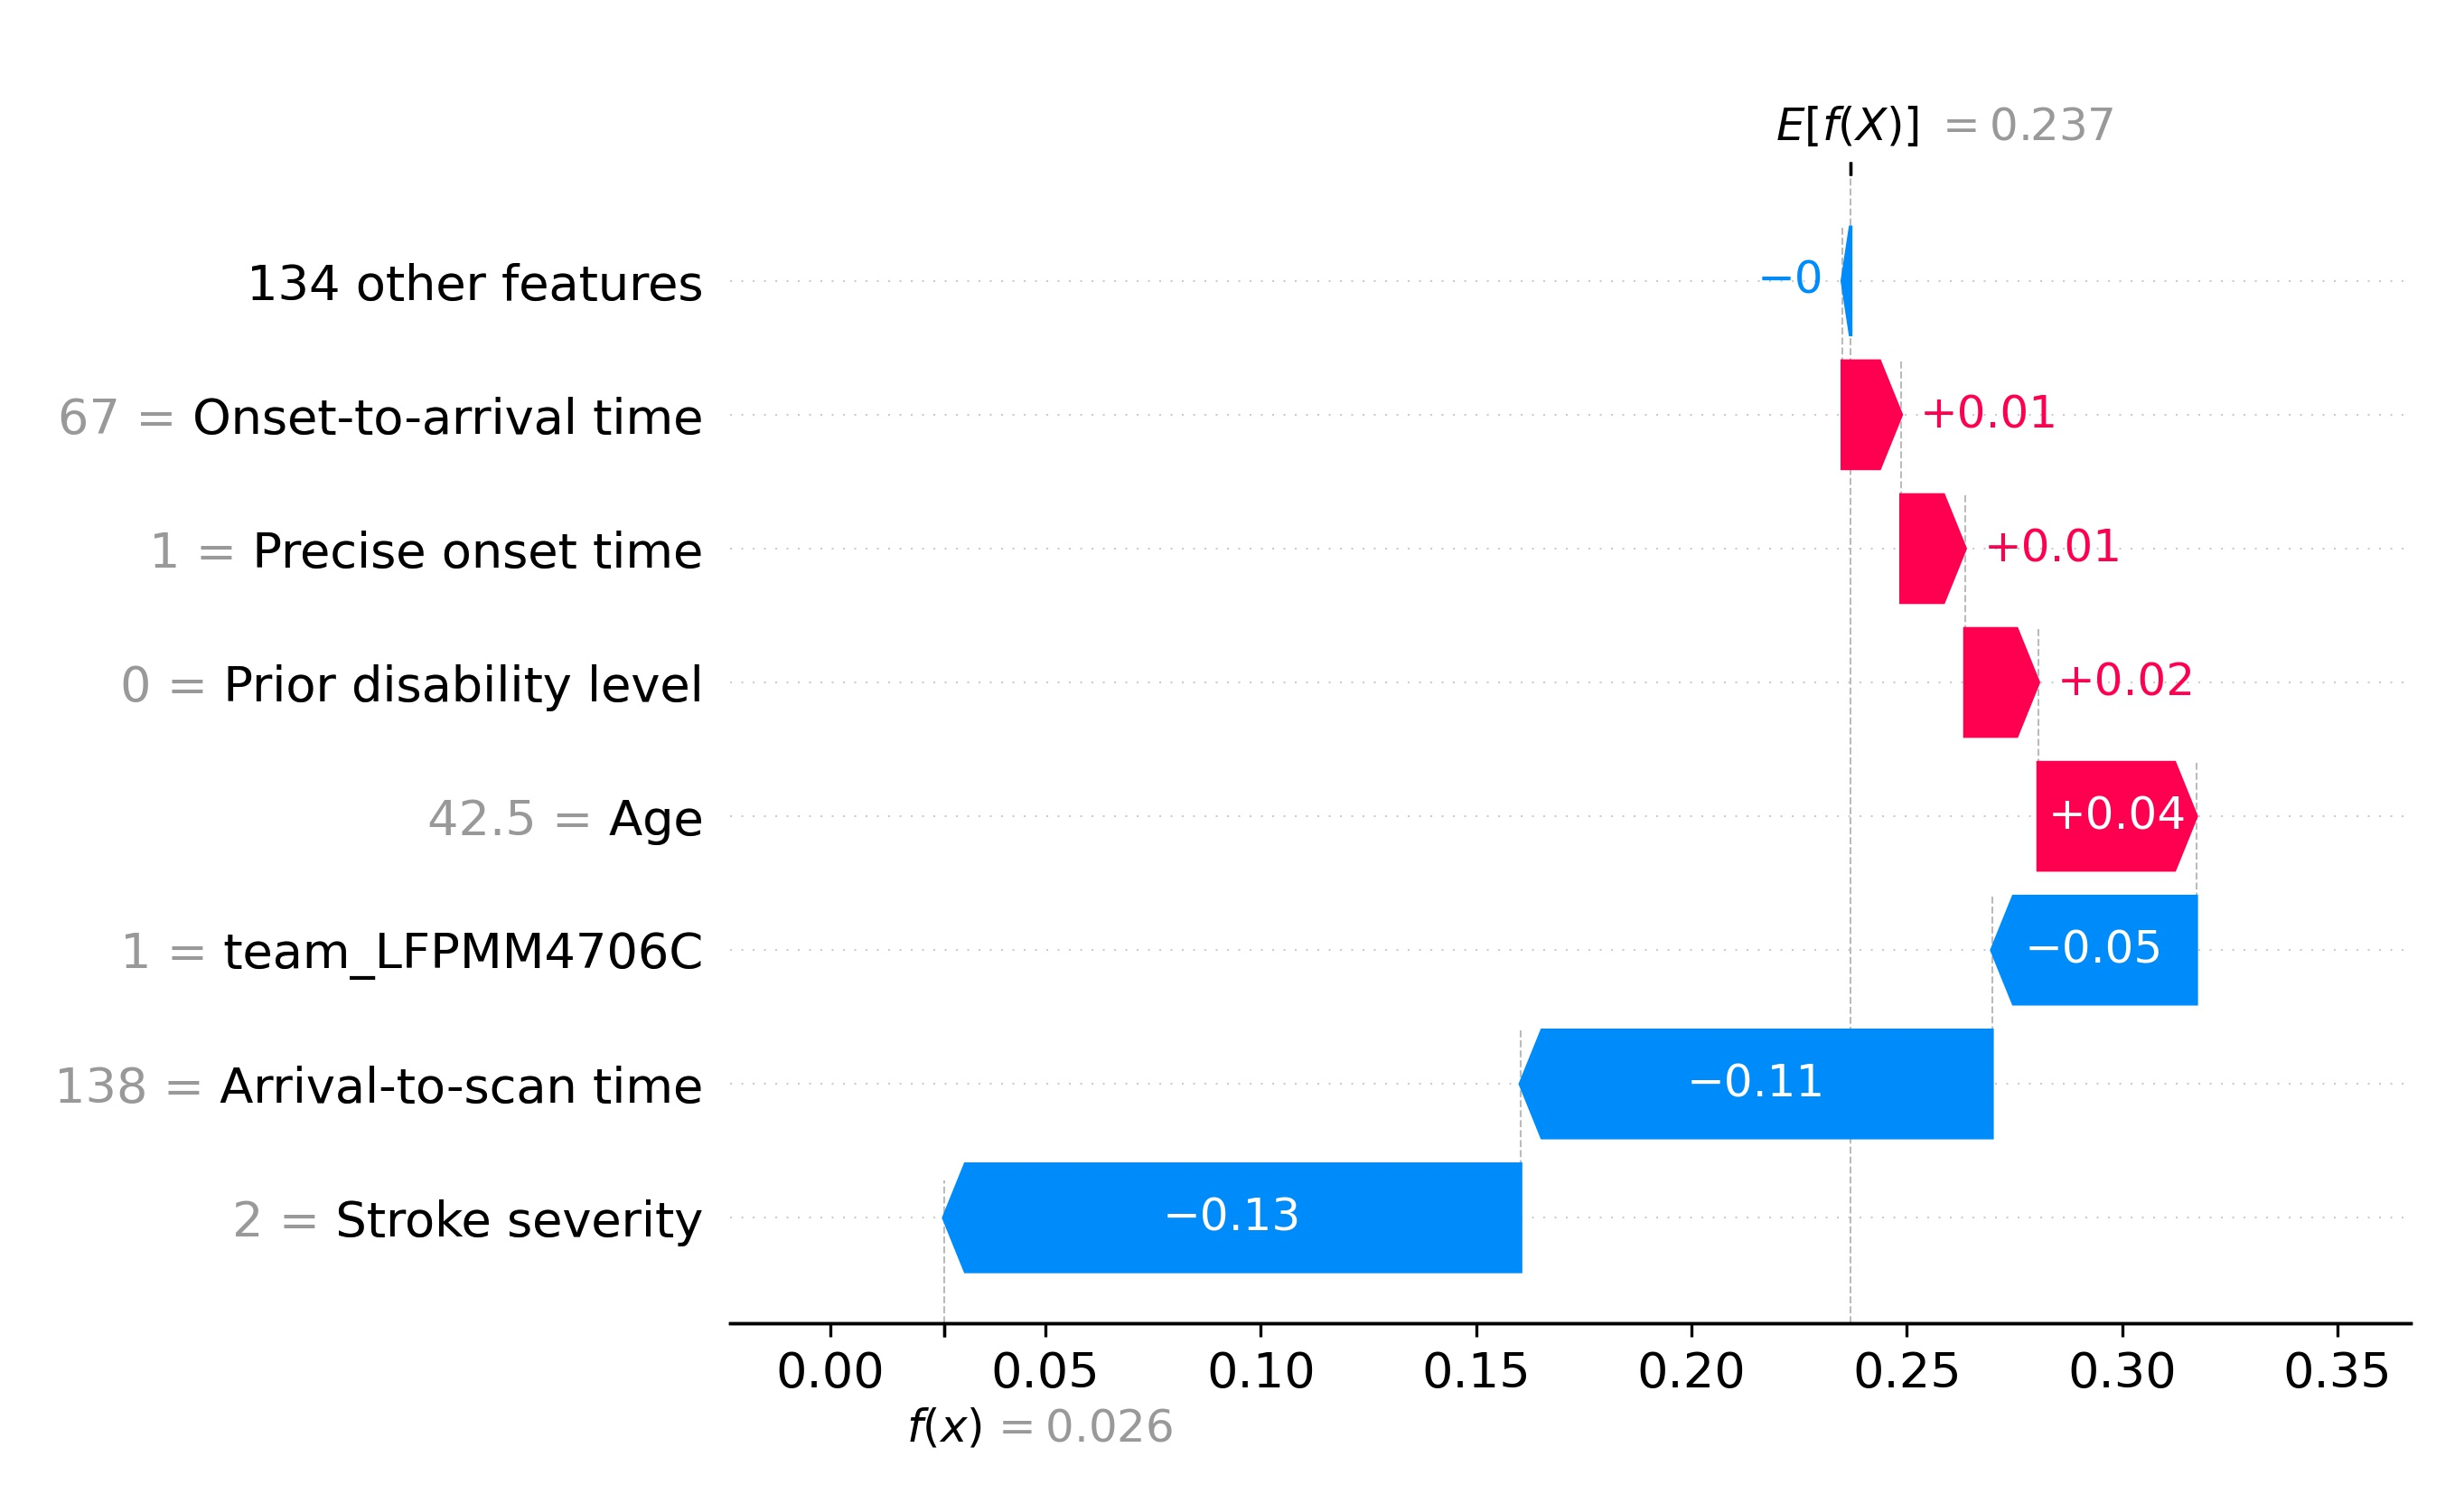
\includegraphics[width=0.8\textwidth]{./images/03_xgb_10_features_waterfall_probability_low}
\caption{Waterfall plot showing the influence of each feature on the predicted probability of a single patient receiving thrombolysis. This example is for a patient with a predicted low probability of receiving thrombolysis.}
\end{figure}

\begin{figure}
\centering
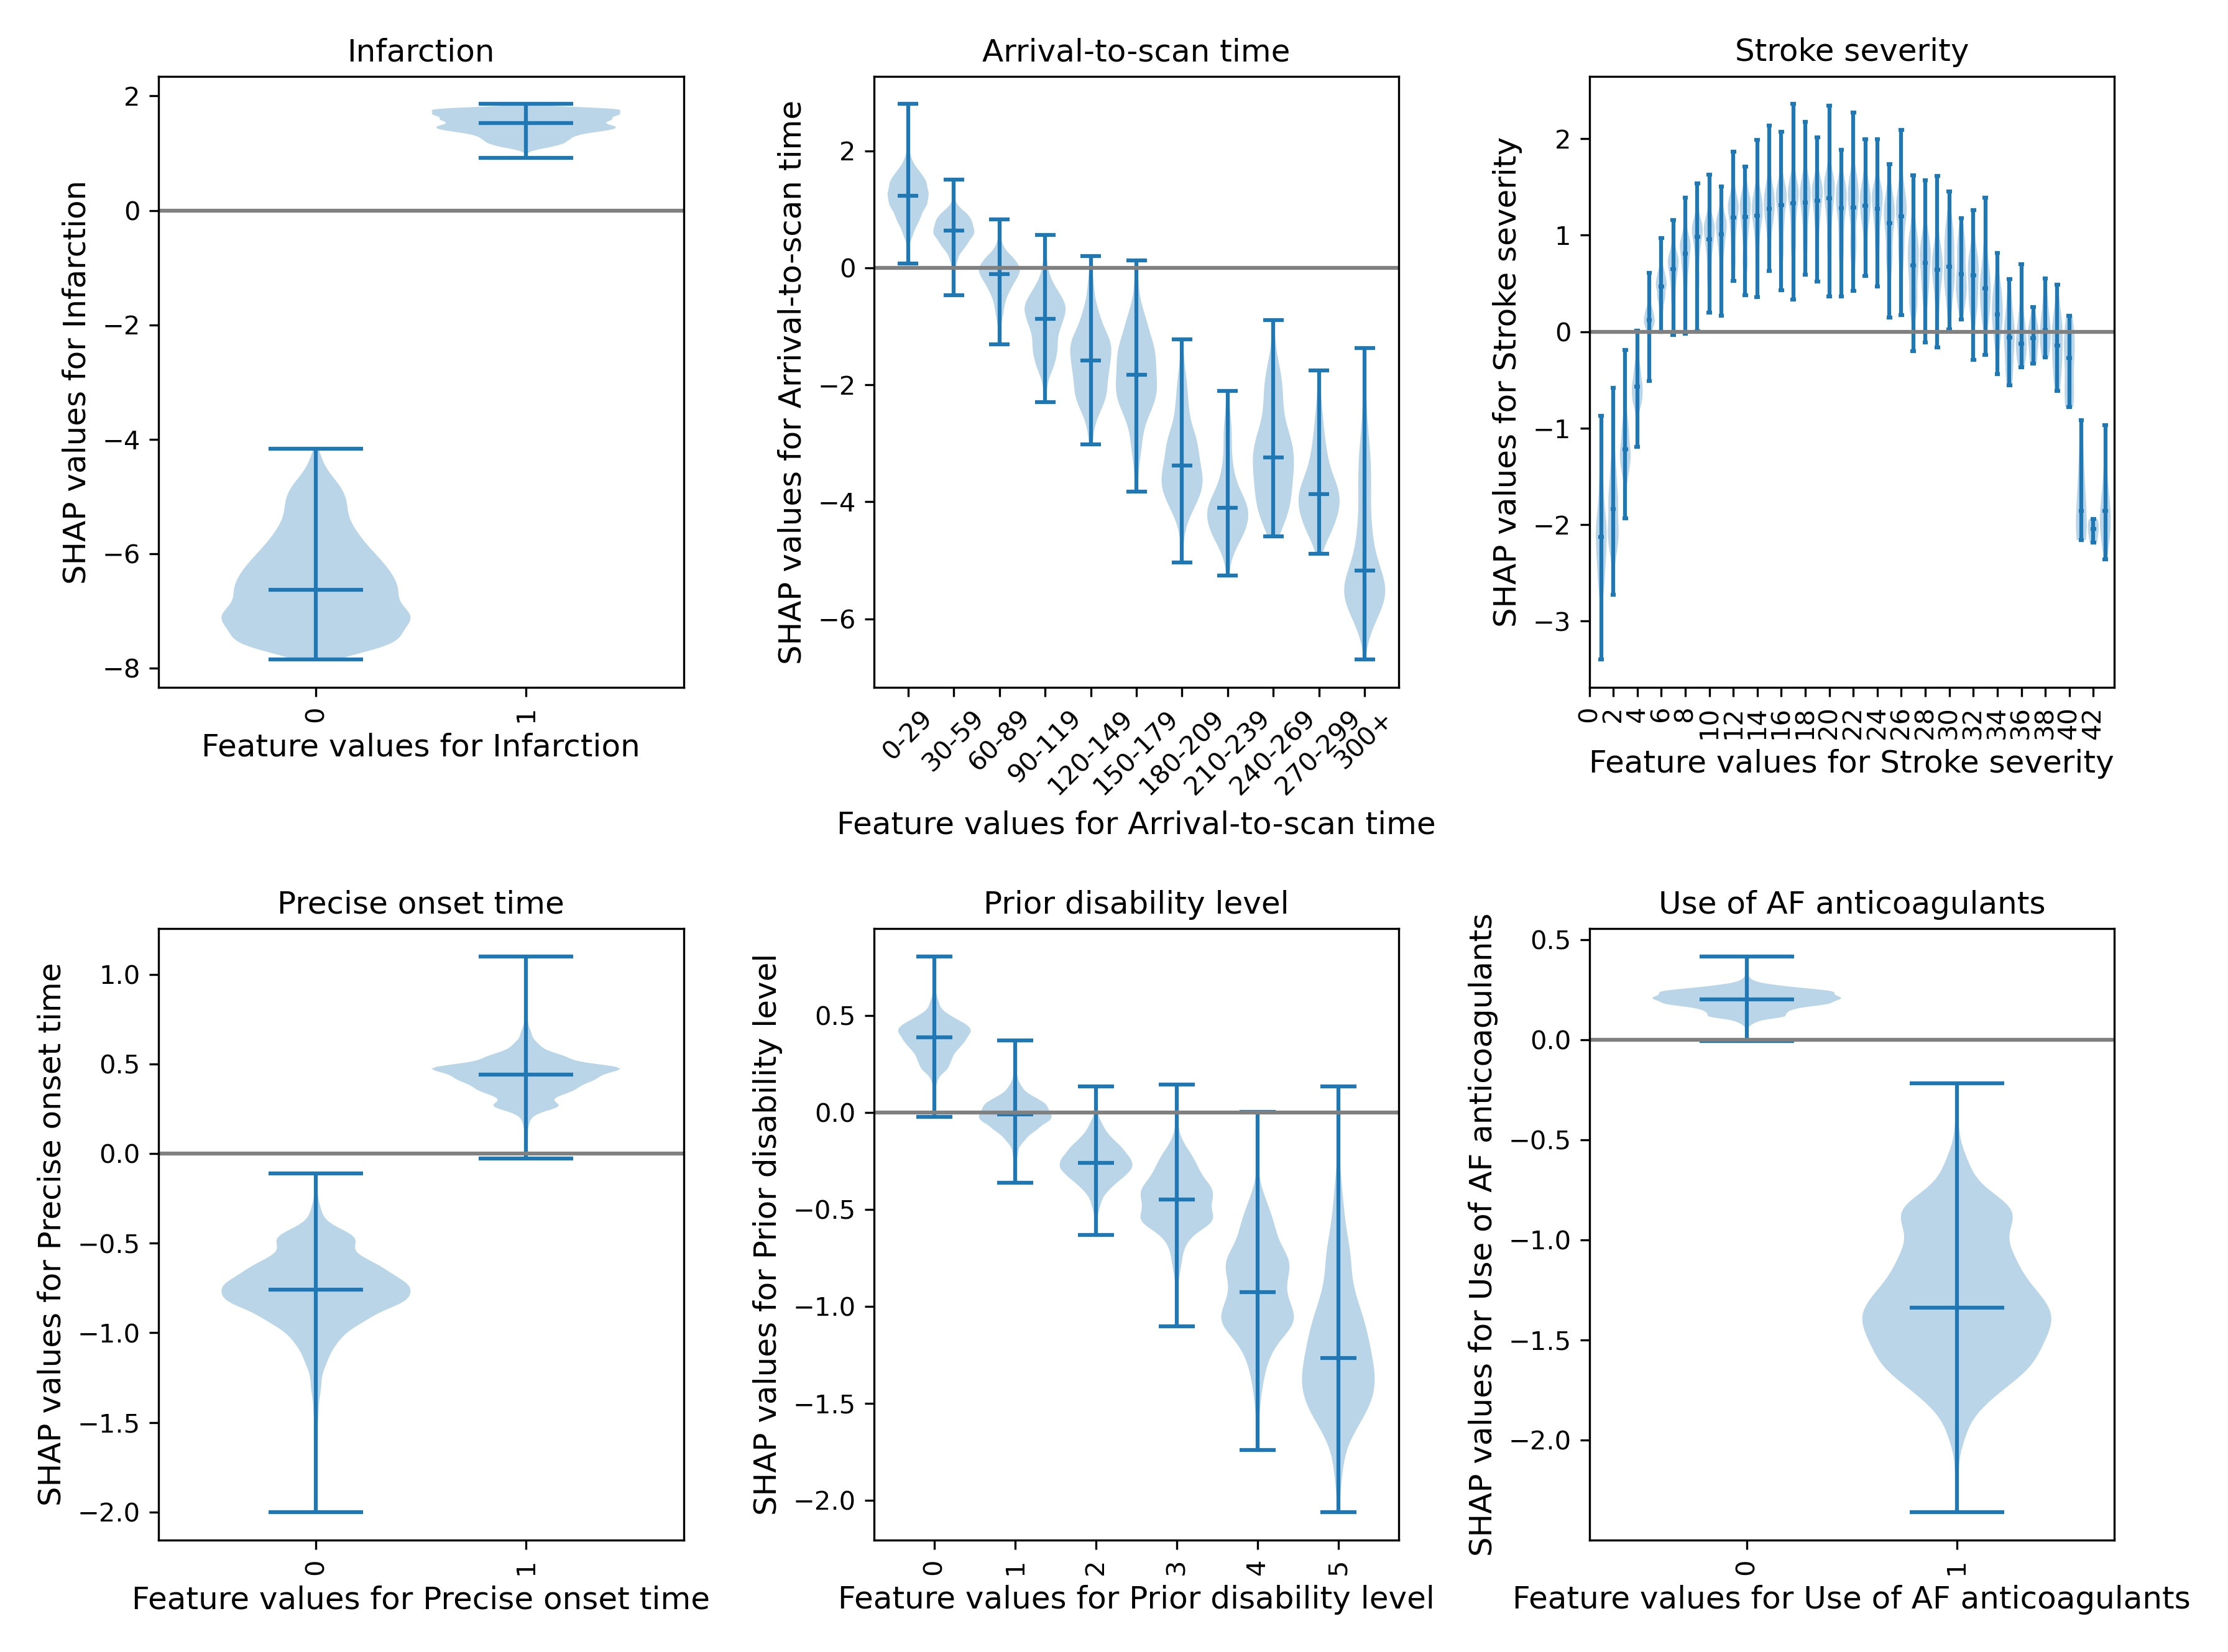
\includegraphics[width=1\textwidth]{./images/03_xgb_10_features_thrombolysis_shap_violin}
\caption{Violin plots showing the relationship between SHAP values and feature values. The horizontal line shows the median SHAP value. SHAP values were taken from the training set of the first of 5 k-fold train/test splits.}
\end{figure}


\begin{figure}
\centering
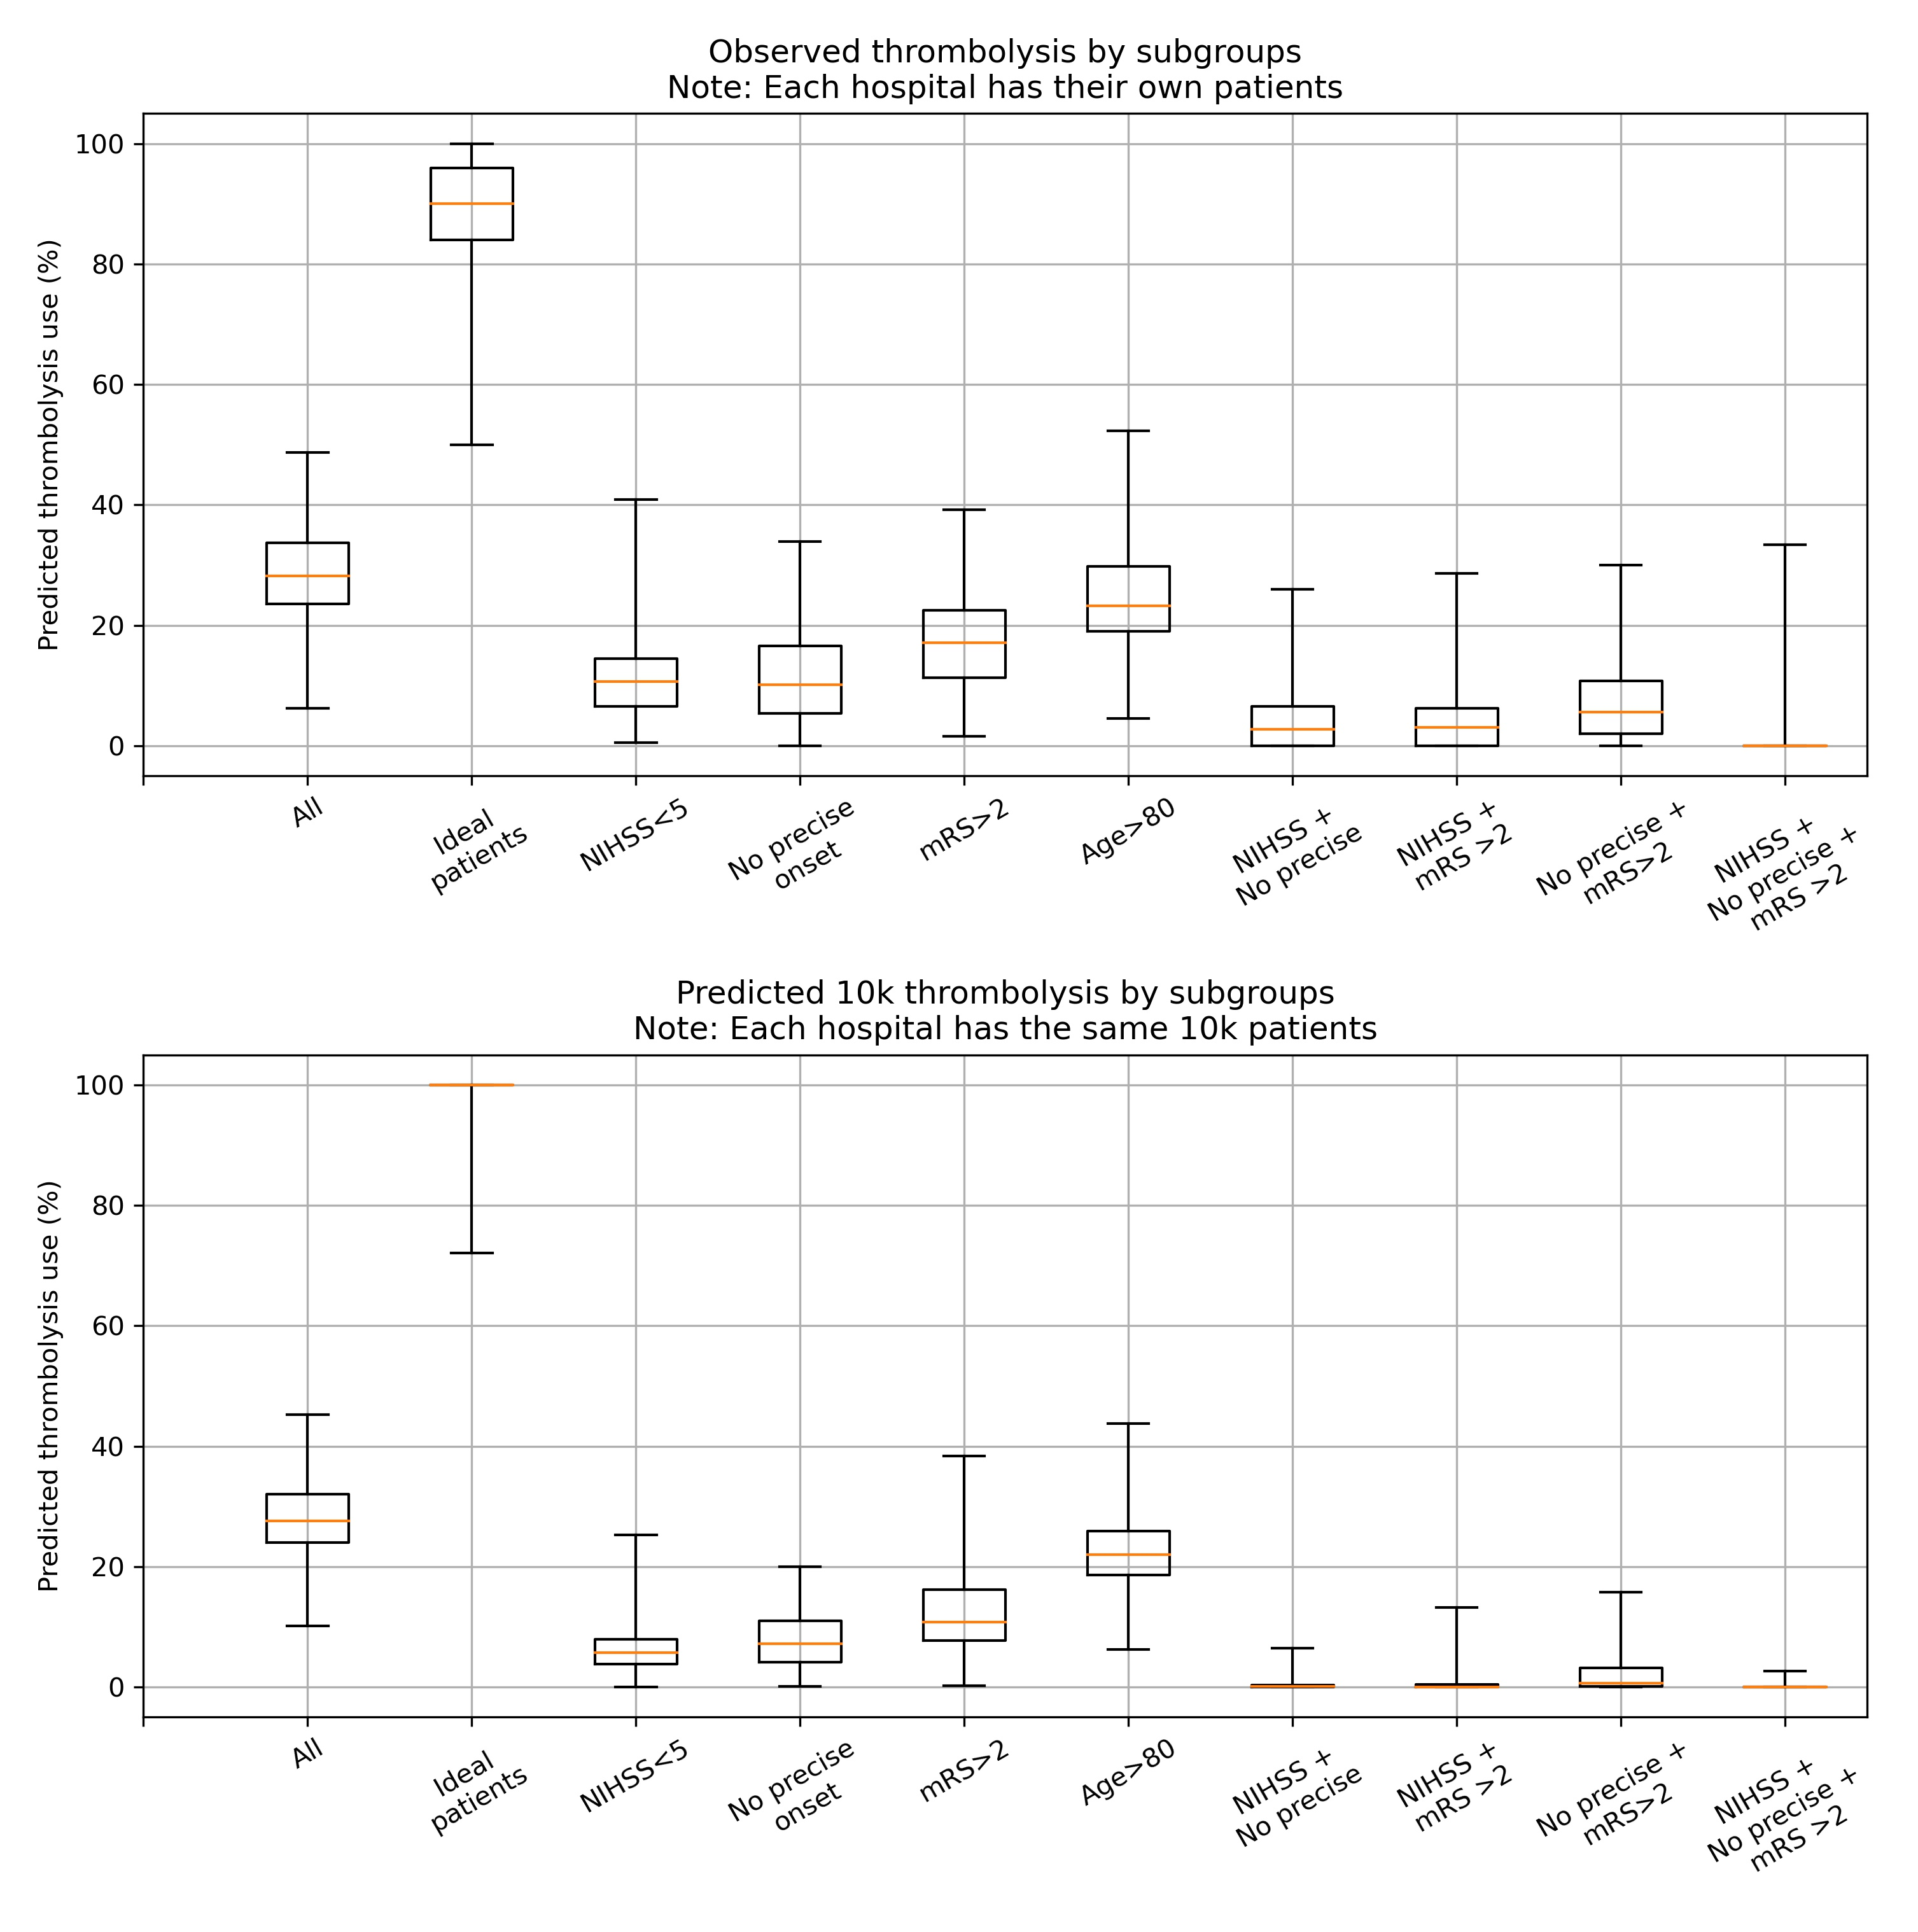
\includegraphics[width=1\textwidth]{./images/15a_actual_vs_modelled_subgroup_violin}
\caption{Boxplot for either observed (top) or predicted (bottom) use of thrombolysis for subgroups of patients.}
\end{figure}

\begin{figure}
\centering
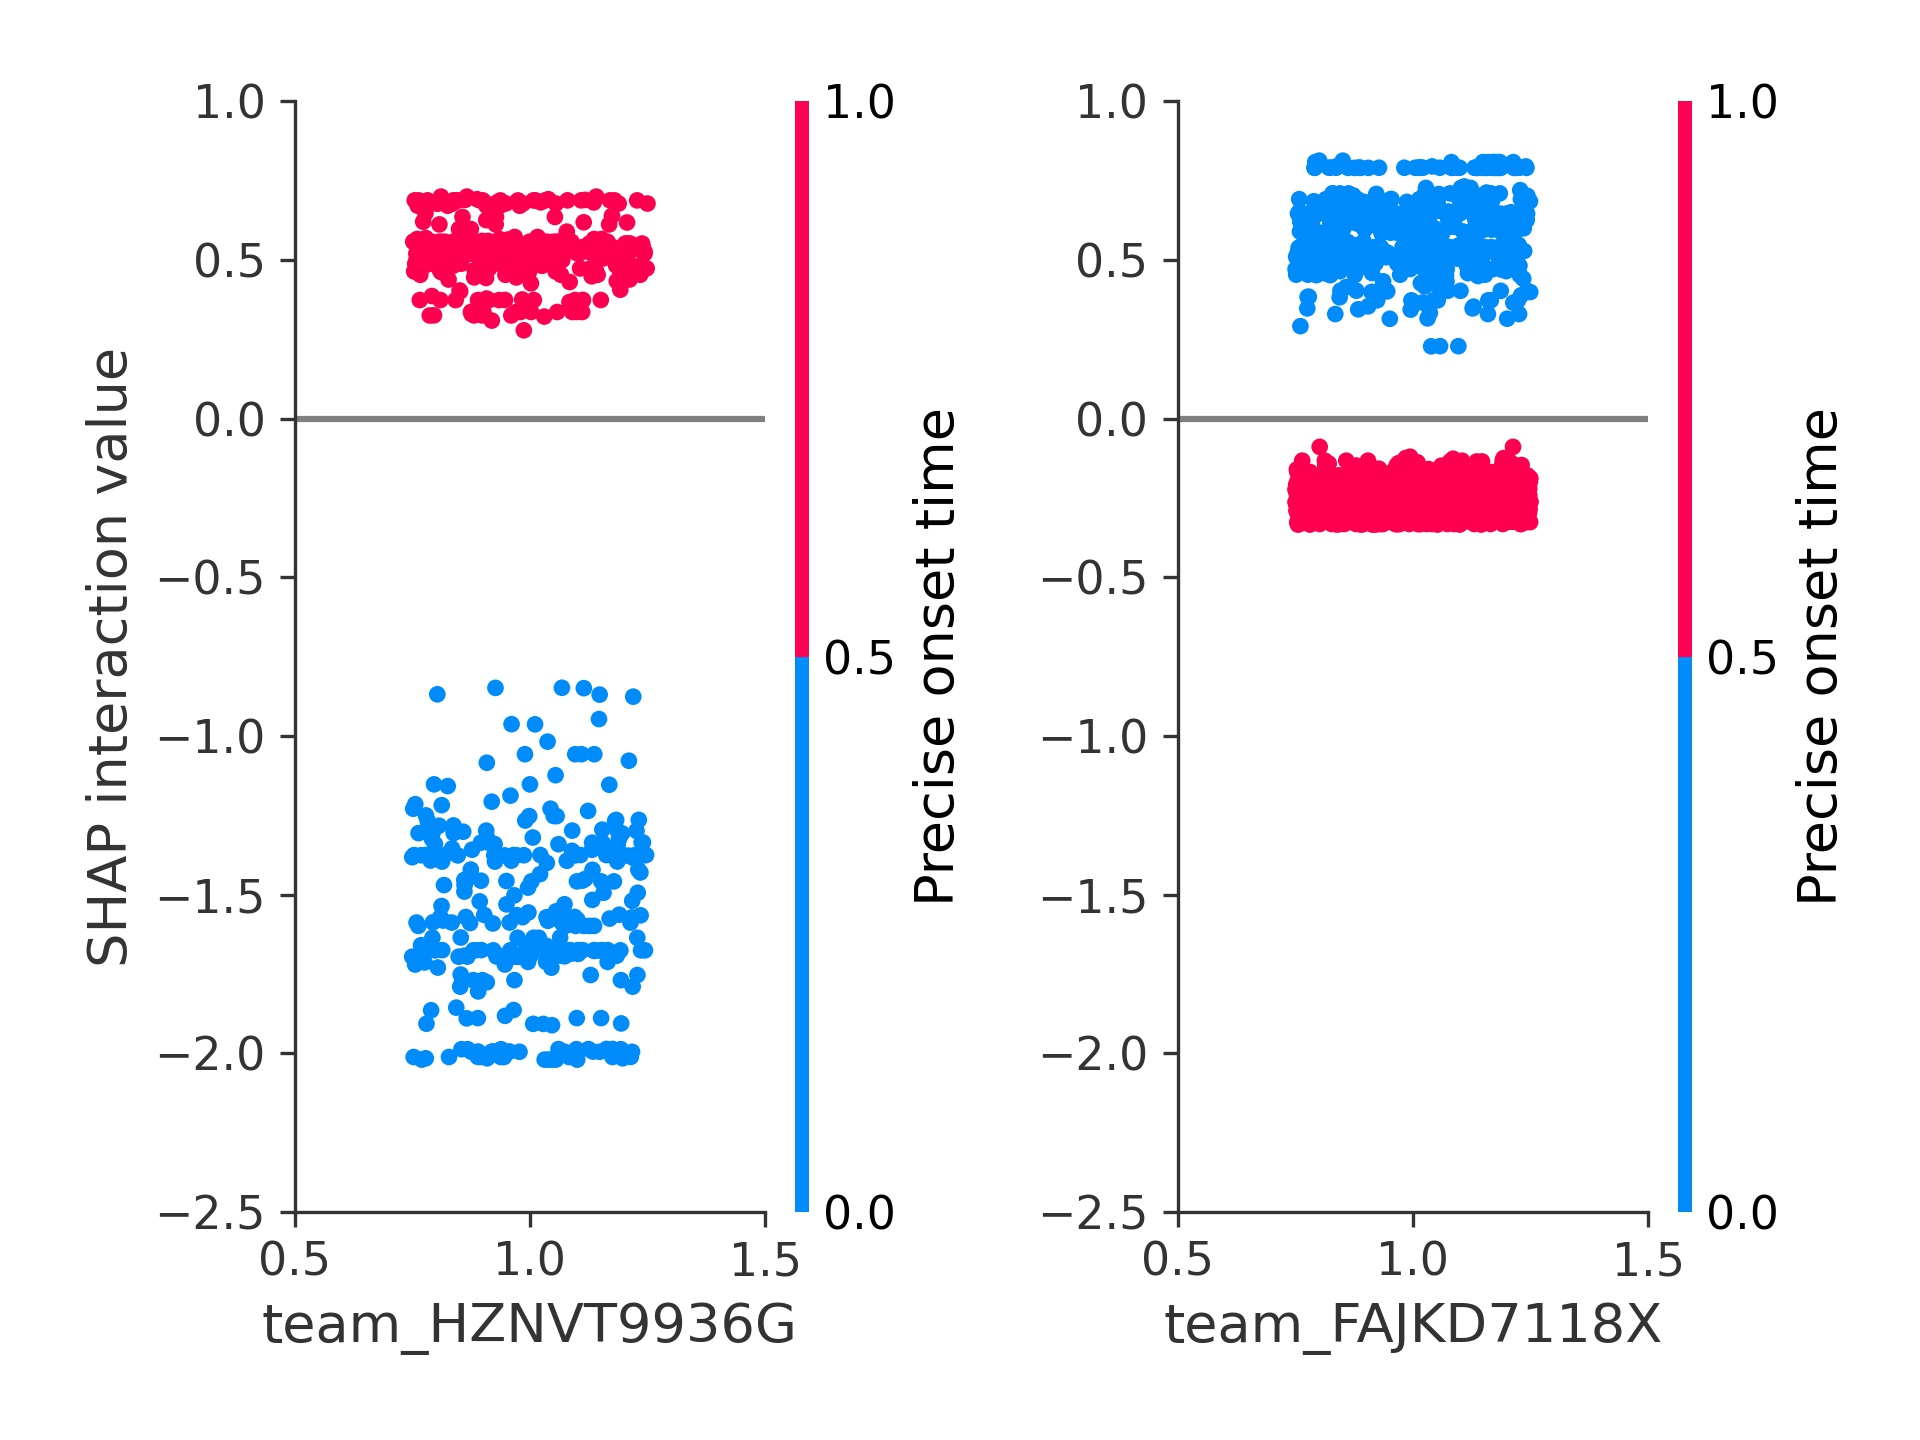
\includegraphics[width=0.7\textwidth]{./images/12aa_onset_time_type_interaction_example}
\caption{SHAP interaction between hospital ID for two teams and whether stroke onset time was known precisely. If a patient attended team HZNVT9936G then SHAP value for having a precise onset time was increased (a strengthening of the main effect of precise onset time). If a patient attended team FAJKD7118X then SHAP value for having a precise onset time was reduced (an attenuation of the main effect of precise onset time).}
\end{figure}

\begin{figure}
\centering
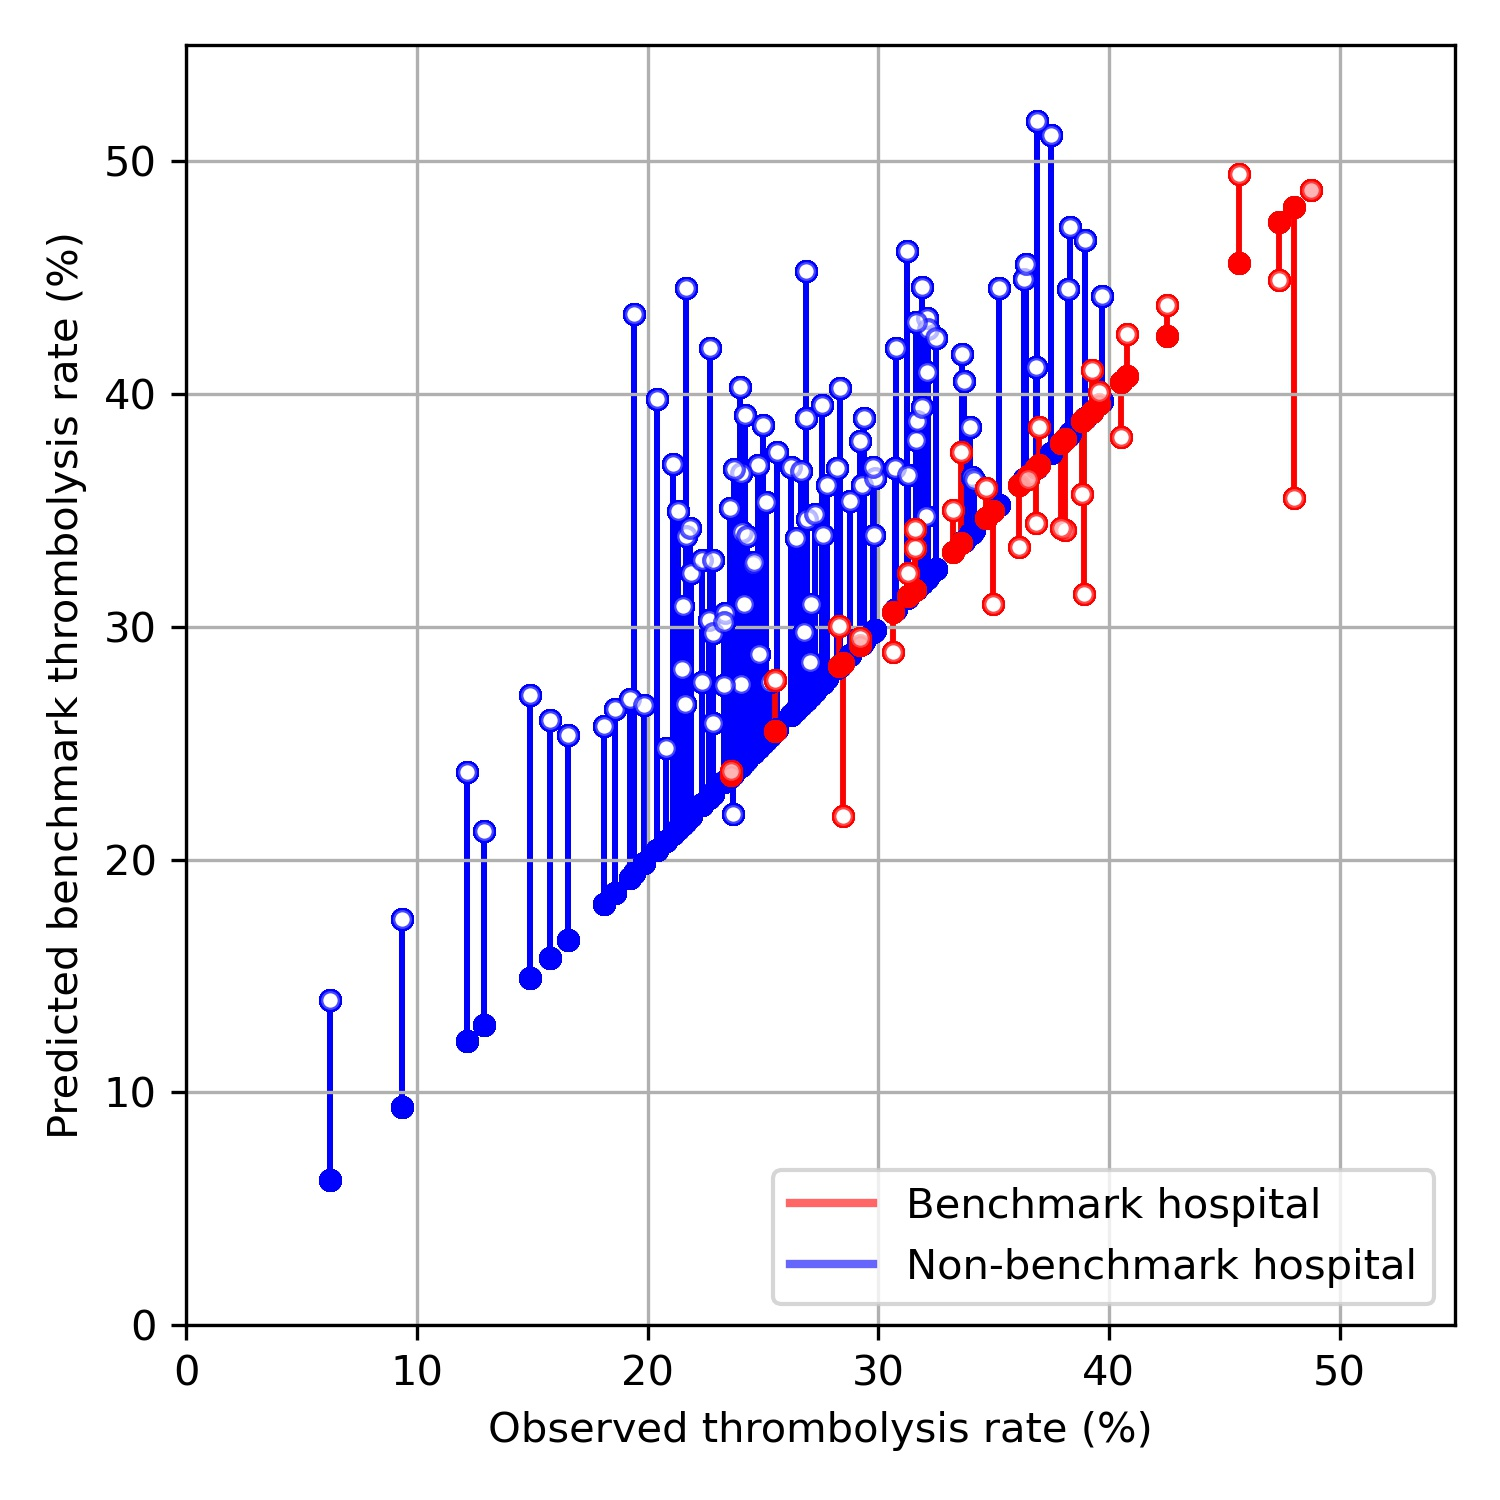
\includegraphics[width=0.7\textwidth]{./images/05_benchmark_thrombolysis_key_features}
\caption{A comparison of observed (actual) thrombolysis rate at each hospital and the predicted thrombolysis rate if decisions were made according to the majority vote of the 30 benchmark hospitals. The solid circle shows the current thrombolysis use, and the open circle shows the thrombolysis use predicted by a majority vote of the benchmark hospitals. The red points are those hospitals that are in the top 30 thrombolysing hospitals (the benchmark set) when 10k cohort thrombolysis use is predicted, with all other hospitals coloured blue.}
\end{figure}











